\documentclass[11pt, a4paper]{article}

% Packages
\usepackage[T1]{fontenc}
\usepackage{lmodern}
\usepackage[margin=2.5cm]{geometry}
\usepackage{graphicx}
\usepackage{booktabs}
\usepackage{array}
\usepackage{tabularx}
\usepackage{caption}
\usepackage{float}
\usepackage{amsmath}
\usepackage{enumitem}
\usepackage{fancyhdr}
\usepackage{listings}
\usepackage{xcolor}
\usepackage{tikz}
\usetikzlibrary{arrows.meta, positioning, calc}
\PassOptionsToPackage{hyphens}{url}
\usepackage[hidelinks]{hyperref}
% Typewriter text that may break at slashes, hyphens, dots and colons
\newcommand{\breakpath}[1]{\nolinkurl{#1}}

% Page style
\pagestyle{fancy}
\fancyhf{}
\fancyhead[L]{\small CSE731 Software Testing: Mid-term Project}
\fancyhead[R]{\small AI-Assisted Unit Testing Pipeline}
\fancyfoot[C]{\small \thepage}
\renewcommand{\headrulewidth}{0.4pt}

\captionsetup{font=small, labelfont=bf}
\setlist{itemsep=2pt}
\renewcommand{\arraystretch}{1.25}

% Code listings
\lstdefinestyle{python}{
    language=Python,
    basicstyle=\ttfamily\footnotesize,
    keywordstyle=\bfseries,
    numbers=left, numberstyle=\tiny, numbersep=6pt,
    frame=single, framerule=0.4pt, rulecolor=\color{black!60},
    breaklines=true, tabsize=4, showstringspaces=false,
    captionpos=b, aboveskip=8pt, belowskip=8pt, xleftmargin=1.5em, framexleftmargin=1.5em,
}
\lstdefinestyle{text}{
    language={},
    basicstyle=\ttfamily\scriptsize,
    frame=single, framerule=0.4pt, rulecolor=\color{black!60},
    breaklines=true, columns=fullflexible, keepspaces=true, showstringspaces=false,
    captionpos=b, aboveskip=8pt, belowskip=8pt,
}
\renewcommand{\lstlistingname}{Listing}

\begin{document}

% Title page
\begin{titlepage}
    \centering
    \vspace*{1.5cm}
    {\large International Institute of Information Technology Bangalore\par}
    \vspace{0.6cm}
    {\large CSE731: Software Testing\par}
    {\normalsize Mid-term Project, Term I (2026/27)\par}
    \vspace{2.5cm}
    \rule{\textwidth}{0.6pt}\par
    \vspace{0.4cm}
    {\LARGE\bfseries AI-Assisted Unit Testing Pipeline\par}
    \vspace{0.3cm}
    {\large Coverage-Driven Test Generation and Verification with Three Agents\par}
    \vspace{0.4cm}
    \rule{\textwidth}{0.6pt}\par
    \vspace{2.5cm}
    {\large Project Report\par}
    \vspace{1.5cm}
    \begin{tabular}{ll}
        \toprule
        \textbf{Name} & \textbf{Roll Number} \\
        \midrule
        Mayank Tanwar & IMT2023012 \\
        Kunal Jindal & IMT2023049 \\
        \bottomrule
    \end{tabular}
    \vfill
    {\large October 2026\par}
\end{titlepage}

\begin{abstract}
This report presents an agentic pipeline for AI-assisted unit testing. For each problem of the MBPP dataset, a Large Language Model (LLM) generates a Python function; a second LLM agent generates unit test cases, consisting of inputs and expected outputs, intended to satisfy a structural coverage criterion selected by the user; and a deterministic executor validates every test case against the dataset's reference solution, executes the valid test cases against the generated function and reports a verdict. The executor additionally constructs the control flow graph of the generated function and verifies whether the executed test cases satisfy the selected criterion. Node, edge, edge-pair and prime path coverage are supported. In the final run, both processed problems received the verdict PASS and met prime path coverage.
\end{abstract}

\tableofcontents
\newpage

% ============================================================================
\section{Introduction}
\label{sec:intro}

The objective of the project is to construct, from first principles, an agentic pipeline that generates unit test cases serving a specific testing goal at the unit level. The pipeline consists of three agents: a code generator, a test case generator and a test case executor.

\paragraph{Test requirement.} The assignment admits three kinds of test requirement. This project implements \textbf{requirement (1), a user-specified coverage criterion}. The user selects one of four graph coverage criteria defined on the control flow graph (CFG) of the generated function: node, edge, edge-pair or prime path coverage. Prime path coverage is the default.

\paragraph{Design constraints.} The pipeline is implemented in plain Python. It does not use retrieval-augmented generation, chain-of-thought prompting or agent frameworks such as LangGraph. Each LLM agent issues a single request consisting of one system message and one user message, and the prompts explicitly forbid the model from presenting its reasoning. The agents are sequenced by ordinary Python control flow.

\paragraph{Structure of the report.} The report follows the five items required by the assignment: the pipeline and the dataset (Section~\ref{sec:pipeline}), the prompts and settings (Section~\ref{sec:prompts}), the formats of the generated code, test cases and verdicts with actual examples (Section~\ref{sec:formats}), the execution results (Section~\ref{sec:results}) and the contribution of each member (Section~\ref{sec:contrib}). Observations and conclusions are given in Sections~\ref{sec:observations} and~\ref{sec:conclusion}.

% ============================================================================
\section{Pipeline and Dataset}
\label{sec:pipeline}

\subsection{Architecture}

The three agents are executed in sequence for every problem, as shown in Figure~\ref{fig:pipeline}. The MBPP reference solution is never shown to either LLM agent; it is used exclusively by the Test Executor to validate the generated test cases.

\begin{figure}[H]
    \centering
    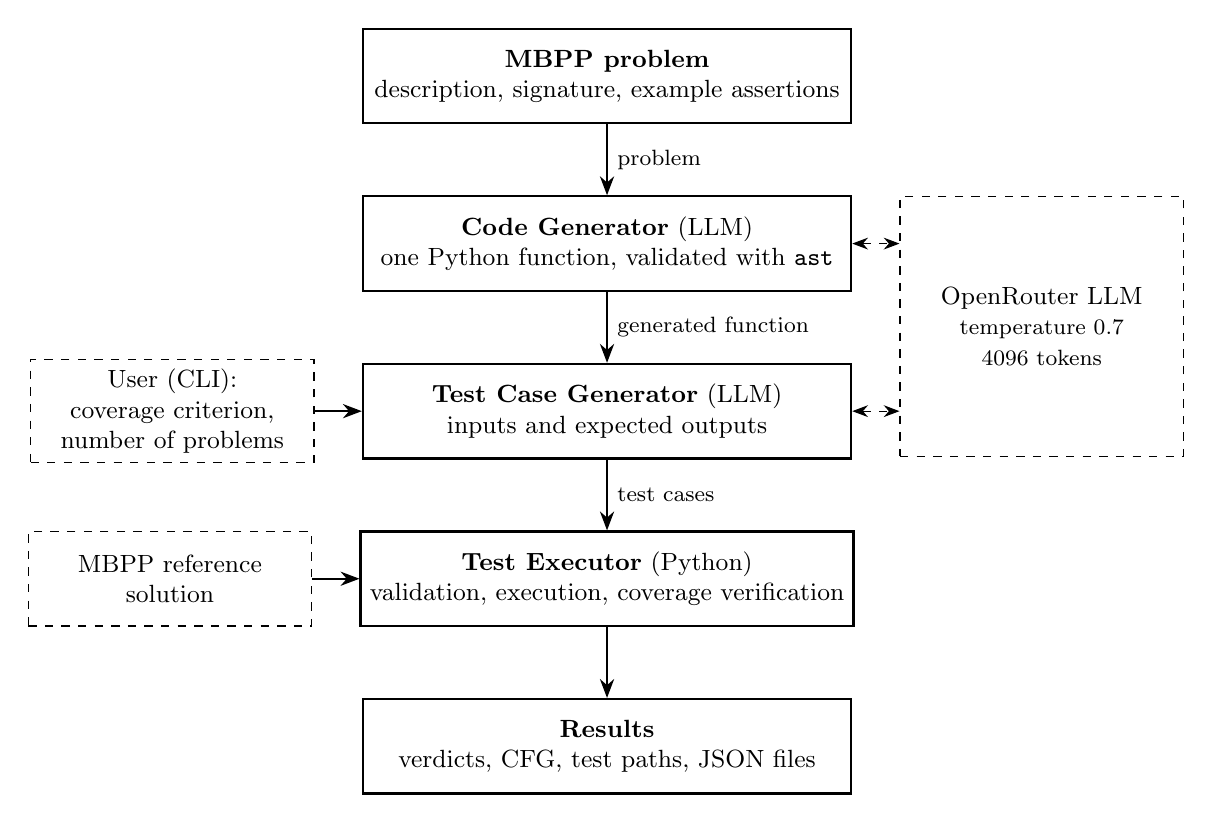
\begin{tikzpicture}[
        node distance=0.9cm,
        box/.style={rectangle, draw=black, thick, minimum width=6.2cm, minimum height=1.2cm, align=center, font=\small},
        side/.style={rectangle, draw=black, dashed, minimum width=3.6cm, minimum height=1.2cm, align=center, font=\small},
        arrow/.style={-{Stealth[length=2.4mm]}, thick},
        lbl/.style={right, font=\footnotesize},
    ]
        \node[box] (mbpp) {\textbf{MBPP problem}\\ description, signature, example assertions};
        \node[box, below=of mbpp] (codegen) {\textbf{Code Generator} (LLM)\\ one Python function, validated with \texttt{ast}};
        \node[box, below=of codegen] (testgen) {\textbf{Test Case Generator} (LLM)\\ inputs and expected outputs};
        \node[box, below=of testgen] (exec) {\textbf{Test Executor} (Python)\\ validation, execution, coverage verification};
        \node[box, below=of exec] (results) {\textbf{Results}\\ verdicts, CFG, test paths, JSON files};
        \node[side, left=0.6cm of testgen] (user) {User (CLI):\\ coverage criterion,\\ number of problems};
        \node[side, left=0.6cm of exec] (ref) {MBPP reference\\ solution};
        \node[side, right=0.6cm of codegen, yshift=-1.05cm, minimum height=3.3cm] (llm) {OpenRouter LLM\\ \footnotesize temperature 0.7\\ \footnotesize 4096 tokens};

        \draw[arrow] (mbpp) to node[lbl] {problem} (codegen);
        \draw[arrow] (codegen) to node[lbl] {generated function} (testgen);
        \draw[arrow] (testgen) to node[lbl] {test cases} (exec);
        \draw[arrow] (exec) to (results);
        \draw[arrow] (user) to (testgen);
        \draw[arrow] (ref) to (exec);
        \draw[{Stealth[length=2mm]}-{Stealth[length=2mm]}, dashed] (codegen.east) to (codegen.east -| llm.west);
        \draw[{Stealth[length=2mm]}-{Stealth[length=2mm]}, dashed] (testgen.east) to (testgen.east -| llm.west);
    \end{tikzpicture}
    \caption{Architecture of the pipeline. Dashed arrows denote LLM requests. The Test Executor discards every test case whose expected output is not reproduced by the reference solution.}
    \label{fig:pipeline}
\end{figure}

\subsection{Dataset}

The pipeline uses the MBPP (Most Basic Python Problems) dataset, configuration \texttt{full}, \texttt{test} split (\breakpath{google-research-datasets/mbpp}), loaded with the Hugging Face \texttt{datasets} library. Each problem provides a natural-language description of the task, a reference solution in Python and three reference \texttt{assert} statements. The assertions determine the name of the function under test and are shown to both LLM agents as example usage. The user specifies the number of problems to process (between 1 and 50, with a default of 1). Problems are processed in dataset order, beginning with task 11.

\subsection{Agents}

\begin{table}[H]
    \centering
    \small
    \begin{tabularx}{\textwidth}{>{\raggedright\arraybackslash}p{3.6cm}>{\raggedright\arraybackslash}p{2.2cm}>{\raggedright\arraybackslash}X>{\raggedright\arraybackslash}X}
        \toprule
        \textbf{Agent} & \textbf{Type} & \textbf{Input} & \textbf{Output} \\
        \midrule
        Code Generator\newline(\texttt{code\_generator.py}) & LLM & Problem description, required signature, MBPP assertions & Exactly one Python function, validated with \texttt{ast} \\
        Test Case Generator\newline(\texttt{test\_case\_generator.py}) & LLM & Description, signature, assertions, generated code, coverage criterion & Test cases consisting of inputs and expected outputs \\
        Test Executor\newline(\texttt{test\_executor.py}, \texttt{coverage\_probe.py}) & Deterministic Python & Test cases, generated code, reference solution & Verdicts per test case and per problem; CFG, test paths and coverage of all four criteria \\
        \bottomrule
    \end{tabularx}
    \caption{The three agents of the pipeline}
\end{table}

\subsection{Processing of a Problem}

\begin{enumerate}
    \item The name and signature of the function under test (for example \texttt{remove\_Occ(s, ch)}) are derived from the reference solution; the name is that of the function invoked in the MBPP assertions.
    \item The \textbf{Code Generator} requests the function from the LLM. The response is accepted only if it consists of exactly one top-level function definition with the required name. Otherwise the LLM is prompted once more, with the reason for the rejection appended to the prompt.
    \item The \textbf{Test Case Generator} requests test cases that satisfy the selected coverage criterion on the generated code. The reference solution is not disclosed to this agent. The response is accepted only if it consists exclusively of test cases in the prescribed format; otherwise the LLM is prompted once more with the reason for the rejection.
    \item The \textbf{Test Executor} parses each test case and executes the reference solution on its input. A test case is valid only if the reference output equals the expected output. The generated function is then executed on every valid test case in a separate process with a time limit of 10 seconds per call, and the assertion \texttt{generated(*args) == expected} is evaluated. Finally, the executor constructs the CFG of the generated function, records the path that each test case follows through it, and determines whether the selected criterion is satisfied.
    \item All prompts, raw LLM responses, generated code, test cases and results are written to the directory \texttt{output/}.
\end{enumerate}

\subsection{Coverage Criteria}

\begin{table}[H]
    \centering
    \small
    \begin{tabularx}{\textwidth}{>{\raggedright\arraybackslash}p{3.2cm}X}
        \toprule
        \textbf{Criterion} & \textbf{Test requirements on the CFG of the generated function} \\
        \midrule
        Node coverage & Every reachable node is executed by at least one test path. \\
        Edge coverage & Every reachable edge is traversed; in particular, each \texttt{if}, \texttt{elif} and \texttt{while} condition evaluates to both True and False, and each loop is both entered and exited. \\
        Edge-pair coverage & Every reachable path of length up to two edges is toured. \\
        Prime path coverage (default) & Every prime path, that is, every simple path that is not a proper sub-path of another simple path, is toured. For loops this includes skipping the loop, executing it once and executing it several times. \\
        \bottomrule
    \end{tabularx}
    \caption{Structural coverage criteria available to the user}
\end{table}

The subsumption relations between these criteria are shown in Figure~\ref{fig:subsumption}. Prime path coverage and edge-pair coverage both subsume edge coverage, and hence node coverage, but neither subsumes the other. In particular, prime path coverage does not subsume edge-pair coverage: if a node $b$ with predecessor $a$ has a self-loop, the edge pair $[a, b, b]$ is a test requirement of edge-pair coverage, but it is not a simple path and is therefore not required by prime path coverage.

\begin{figure}[H]
    \centering
    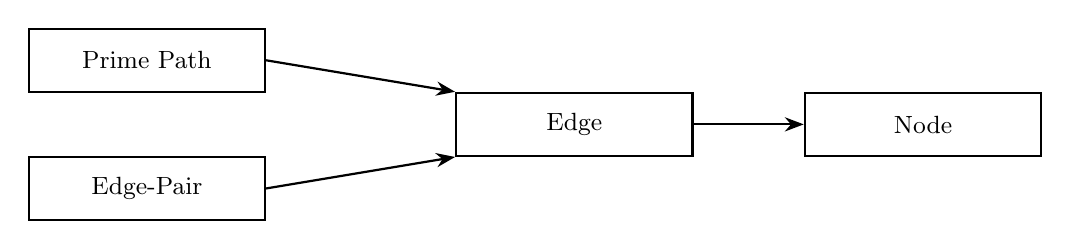
\begin{tikzpicture}[
        crit/.style={rectangle, draw=black, thick, minimum width=3cm, minimum height=0.8cm, font=\small},
        imp/.style={-{Stealth[length=2.4mm]}, thick},
    ]
        \node[crit] (pp) {Prime Path};
        \node[crit, below=0.8cm of pp] (ep) {Edge-Pair};
        \coordinate (mid) at ($(pp.east)!0.5!(ep.east)$);
        \node[crit, right=2.4cm of mid] (e) {Edge};
        \node[crit, right=1.4cm of e] (n) {Node};
        \draw[imp] (pp.east) to (e.north west);
        \draw[imp] (ep.east) to (e.south west);
        \draw[imp] (e) to (n);
    \end{tikzpicture}
    \caption{Subsumption hierarchy of the supported criteria (an arrow from A to B means that A subsumes B)}
    \label{fig:subsumption}
\end{figure}

\subsection{Automatic Verification of the Coverage Criterion}
\label{sec:verification}

The LLM is instructed to reason about the CFG of the generated function, but there is no guarantee that it does so correctly. The Test Executor therefore verifies the criterion independently (\texttt{coverage\_probe.py}) in four steps.
\begin{enumerate}
    \item \textbf{Control flow graph.} The generated function is parsed with the \texttt{ast} module and its CFG is constructed. Consecutive statements are grouped into basic blocks, which form the nodes of the graph, and a synthetic exit node is added as the final node. Each \texttt{if}, \texttt{elif} and \texttt{while} condition forms a single decision node (a compound condition such as \texttt{a or b} is not decomposed), and every loop header is a node of its own. The constructs \texttt{break}, \texttt{continue}, \texttt{return}, loop \texttt{else} clauses and \texttt{try}/\texttt{except} are modelled; nested helper functions are treated as single statements.
    \item \textbf{Test paths.} In the same pass, a copy of the function is instrumented with probe calls. The input of every valid test case is executed on this copy, which records the sequence of CFG nodes visited, that is, the test path. Each recursive call yields a separate test path.
    \item \textbf{Test requirements.} For all four criteria the test requirements are derived from the CFG following Ammann and Offutt. Prime paths are obtained by enumerating all simple paths and retaining the maximal ones; the implementation reproduces the eight prime paths of the textbook example.
    \item \textbf{Touring.} A test requirement is covered if it occurs as a contiguous sub-path of at least one test path. The selected criterion is reported as met if and only if all of its test requirements are covered.
\end{enumerate}
The verdict is always computed on the original, uninstrumented function; the instrumented copy serves only to record test paths. Whether a path is executable cannot be decided automatically in general, so an uncovered requirement may be infeasible. Uncovered requirements are therefore listed explicitly for inspection.

\subsection{Technology}

\begin{table}[H]
    \centering
    \small
    \begin{tabular}{ll}
        \toprule
        \textbf{Component} & \textbf{Technology} \\
        \midrule
        Language & Python 3 (tested with versions 3.9 and 3.14) \\
        LLM API & OpenRouter, free models \\
        Command-line interface & \texttt{argparse} and Rich; interactive and batch modes (\texttt{cli.py}) \\
        Dataset & Hugging Face \texttt{datasets} \\
        Code validation and parsing & Python \texttt{ast} module \\
        Test execution & \texttt{multiprocessing} worker processes, one time limit per call \\
        Coverage verification & CFG construction from the AST, recorded test paths \\
        \bottomrule
    \end{tabular}
    \caption{Technology used in the implementation}
\end{table}

% ============================================================================
\section{Prompts and Settings}
\label{sec:prompts}

\subsection{Settings}

Both LLM agents use the same settings, listed in Table~\ref{tab:settings}. Each request contains one system message and one user message, without conversation history. For every problem, the prompts, the model that produced each response and the raw responses are stored in \texttt{code\_gen\_prompts.json} and \texttt{test\_gen\_prompts.json}.

\begin{table}[H]
    \centering
    \small
    \begin{tabularx}{\textwidth}{>{\raggedright\arraybackslash}p{4.6cm}X}
        \toprule
        \textbf{Parameter} & \textbf{Value} \\
        \midrule
        API endpoint & \breakpath{https://openrouter.ai/api/v1/chat/completions} \\
        Primary model & \breakpath{cohere/north-mini-code:free} \\
        Fallback models & \breakpath{google/gemma-4-31b-it:free}, \breakpath{google/gemma-4-26b-a4b-it:free}, \breakpath{qwen/qwen3.8-27b:free}, \breakpath{nvidia/nemotron-3.5-lightning:free}, \breakpath{nvidia/nemotron-3-ultra-550b-a55b:free} \\
        Temperature & 0.7 \\
        Maximum output tokens & 4096 \\
        Other sampling parameters & Provider defaults \\
        Messages per request & One system message and one user message \\
        Re-prompts & One per agent, including the reason for the rejection, if the response violates the output format \\
        Truncated responses & Discarded; the next fallback model is used \\
        Time limit per call & 10 seconds \\
        Maximum number of test cases requested & 20 \\
        User-selectable settings & Coverage criterion (default: prime path coverage) and number of problems (1 to 50, default: 1) \\
        \bottomrule
    \end{tabularx}
    \caption{LLM and execution settings}
    \label{tab:settings}
\end{table}

When a model is rate-limited (HTTP 429), the client waits for the \texttt{Retry-After} interval and repeats the request once. When a model is unavailable (HTTP 404, 502 or 503), or when its response was truncated at the token limit (\texttt{finish\_reason} equal to \texttt{"length"}), the next fallback model is used. Only the final \texttt{content} field of a response is used; reasoning fields returned by some models are ignored.

\subsection{Code Generator Prompts}

The system prompt of the Code Generator is shown in Listing~\ref{lst:codesys}, and the user prompt for task 11 in Listing~\ref{lst:codeuser}. The user prompt is constructed from the problem description, the required signature and the three MBPP assertions.

\begin{lstlisting}[style=text, caption={System prompt of the Code Generator}, label={lst:codesys}]
You are a Python code generator in an automated unit-testing pipeline. Your response is loaded by a program that calls your function with test inputs, so it must be exactly one Python 3 function definition and nothing else.

Rules:
1. Write exactly one function, with exactly the name and parameters given in the user message.
2. Put any import statements and helper functions INSIDE the function body. Nothing may appear before or after the function.
3. The function must return its result. Do not print, do not read input(), and do not include example usage, test cases or assert statements.
4. Do not write any text outside the function: no reasoning or thinking process, no explanations and no markdown code fences (```).
5. The first line of your response must be `def <function name>(`.
\end{lstlisting}

\begin{lstlisting}[style=text, caption={User prompt of the Code Generator for task 11}, label={lst:codeuser}]
Problem description:
Write a python function to remove first and last occurrence of a given character from the string.

Required function signature:
def remove_Occ(s, ch):

Example usage (shows the expected behaviour):
assert remove_Occ("hello","l") == "heo"
assert remove_Occ("abcda","a") == "bcd"
assert remove_Occ("PHP","P") == "H"

Write the function now.
\end{lstlisting}

The response is accepted only if it parses as exactly one top-level function definition with the required name. Otherwise it is rejected, and the request is repeated once with the following sentence appended to the user prompt: \emph{``Your previous response was rejected because \textless reason\textgreater. Respond again with only the function definition.''} A markdown fence enclosing an otherwise valid response is removed, and the removal is recorded in the field \texttt{markdown\_fence\_removed}.

\subsection{Test Case Generator Prompts}

The system prompt of the Test Case Generator consists of four parts: the role, the test requirement, the rule for expected outputs and the output format. Listing~\ref{lst:testsys} shows the complete system prompt for prime path coverage.

\begin{lstlisting}[style=text, caption={System prompt of the Test Case Generator for prime path coverage}, label={lst:testsys}]
You are a unit-test generator in an automated software testing pipeline. You generate unit test cases for a Python function: the inputs of each test case and the output the function is expected to return.

TEST REQUIREMENT
Prime Path Coverage of the code under test.
Consider the control flow graph (CFG) of the function under test: nodes are basic blocks (maximal sequences of statements executed together) and edges are the possible transfers of control between them, including both outcomes of every decision and the entry/exit of every loop. A prime path is a simple path (no node appears twice, except that the first and last node may be the same) that is not a proper sub-path of any other simple path. Choose inputs so that every feasible prime path is toured by at least one test case. For every loop this includes inputs that skip the loop, run it exactly once and run it several times.
Use at most 20 test cases.

EXPECTED OUTPUTS
The expected output of a test case is the value that a CORRECT solution of the problem returns, as defined by the problem description and the example usage. The code under test may contain bugs: use it only to choose inputs for the coverage requirement, never to decide the expected output.

OUTPUT FORMAT
Your response is read by a program, not by a person. It must START with <OPEN> and END with <CLOSE>, and contain nothing except the test cases: no reasoning or thinking process, no explanation, no restating of these rules, no markdown. Any other text makes the whole response invalid.
- Each test case is TWO blocks: <OPEN>arguments<CLOSE><OPEN>expected output<CLOSE>.
- The arguments block contains the arguments for ONE call of the function, in the same order as the function parameters, separated by the $ character.
- The expected output block contains the single value the function must return for those arguments.
- Every argument and every expected output must be a Python literal: int, float, str, bytes, bool, None, list, tuple, dict or set.
- Every string MUST be enclosed in double quotes, including strings inside lists, tuples, sets and dicts: write "abc_def", never abc_def. An unquoted word is rejected as an invalid test case.
- String values must never contain the text <OPEN> or <CLOSE>.
- Write the test cases one after another: <OPEN>arguments 1<CLOSE><OPEN>expected output 1<CLOSE><OPEN>arguments 2<CLOSE><OPEN>expected output 2<CLOSE>...
- Do NOT write the function name, assert statements, variable names, comments, explanations or markdown. Your entire response must consist only of the test cases.
- Only use inputs that are valid for the problem description.

EXAMPLES
For def remove_Occ(s, ch):  <OPEN>"hello"$"l"<CLOSE><OPEN>"heo"<CLOSE><OPEN>"abcda"$"a"<CLOSE><OPEN>"bcd"<CLOSE><OPEN>""$"x"<CLOSE><OPEN>""<CLOSE>
For def is_snake_case(text):  <OPEN>"abc_def"<CLOSE><OPEN>True<CLOSE><OPEN>"Abc_def"<CLOSE><OPEN>False<CLOSE>
For def max_of_list(nums):  <OPEN>[3, 1, 2]<CLOSE><OPEN>3<CLOSE><OPEN>[-5]<CLOSE><OPEN>-5<CLOSE>
For def merge_dicts(d1, d2):  <OPEN>{"a": 1}${"b": 2}<CLOSE><OPEN>{"a": 1, "b": 2}<CLOSE>
\end{lstlisting}

Only the \texttt{TEST REQUIREMENT} block depends on the selected criterion. Each variant begins with the CFG definition shown in Listing~\ref{lst:testsys}, followed by the text in Table~\ref{tab:requirements}.

\begin{table}[H]
    \centering
    \small
    \begin{tabularx}{\textwidth}{>{\raggedright\arraybackslash}p{2.6cm}X}
        \toprule
        \textbf{Criterion} & \textbf{Requirement text following the CFG definition} \\
        \midrule
        Node & Choose inputs so that every reachable node of the CFG (every statement) is executed by at least one test case. \\
        Edge & Choose inputs so that every reachable edge of the CFG is traversed by at least one test case: every if / elif / while condition must evaluate to both True and False, and every loop must be both entered and exited. \\
        Edge-pair & Choose inputs so that every reachable path of length up to two edges (every pair of consecutive edges, and every single edge) of the CFG is toured by at least one test case. \\
        Prime path & The definition of prime paths and the instruction shown in Listing~\ref{lst:testsys}. \\
        \bottomrule
    \end{tabularx}
    \caption{Test requirement for each coverage criterion}
    \label{tab:requirements}
\end{table}

The user prompt (Listing~\ref{lst:testuser}) contains the generated code, to which the coverage criterion refers. The reference solution is not included.

\begin{lstlisting}[style=text, caption={User prompt of the Test Case Generator for task 11}, label={lst:testuser}]
Problem description:
Write a python function to remove first and last occurrence of a given character from the string.

Function under test:
def remove_Occ(s, ch):

Example usage (shows the expected behaviour):
assert remove_Occ("hello","l") == "heo"
assert remove_Occ("abcda","a") == "bcd"
assert remove_Occ("PHP","P") == "H"

Code under test (the coverage requirement refers to this code; it may contain bugs):
```python
def remove_Occ(s, ch):
    first = s.find(ch)
    if first == -1:
        return s
    last = s.rfind(ch)
    if first == last:
        return s[:first] + s[first+1:]
    else:
        return s[:first] + s[first+1:last] + s[last+1:]
```

Respond with the test cases only: start with <OPEN> and end with <CLOSE>.
\end{lstlisting}

The response is accepted only if it consists exclusively of test cases: it must begin with \texttt{<OPEN>}, end with \texttt{<CLOSE>}, contain no text between the blocks and contain an even number of blocks (one block of arguments and one block with the expected output per test case). A markdown fence enclosing an otherwise valid response is tolerated. Any other response is rejected, and the request is repeated once with the reason appended, for example: \emph{``Your previous response was rejected because it does not start with \texttt{<OPEN>} (it starts with "Here's a thinking process: \ldots"). Respond again with ONLY the test cases: start with \texttt{<OPEN>}, end with \texttt{<CLOSE>}, and write nothing else.''} If the second response is also rejected, test generation for the problem fails and its verdict is \texttt{NOT RUN}.

% ============================================================================
\section{Format of the Code, Test Cases and Verdicts}
\label{sec:formats}

The generated code is a single Python function, each test case is a pair of tagged blocks containing Python literals, and the verdicts are stored as one JSON record per problem. All examples in this section are actual outputs of the final pipeline run for task 11.

\subsection{Generated Code}
\label{sec:codeformat}

The generated code consists of exactly one function with the required name and parameters; imports and helper functions, if any, are placed inside the function body. Listing~\ref{lst:gencode} shows the raw LLM response for task 11, which was accepted at the first attempt, and Listing~\ref{lst:refcode} the MBPP reference solution, which is used only to validate test cases.

\begin{lstlisting}[style=python, caption={Generated code for task 11 (\texttt{generated\_code.py})}, label={lst:gencode}]
def remove_Occ(s, ch):
    first = s.find(ch)
    if first == -1:
        return s
    last = s.rfind(ch)
    if first == last:
        return s[:first] + s[first+1:]
    else:
        return s[:first] + s[first+1:last] + s[last+1:]
\end{lstlisting}

\begin{lstlisting}[style=python, caption={MBPP reference solution for task 11 (\texttt{reference\_code.py})}, label={lst:refcode}]
def remove_Occ(s,ch):
    for i in range(len(s)):
        if (s[i] == ch):
            s = s[0 : i] + s[i + 1:]
            break
    for i in range(len(s) - 1,-1,-1):
        if (s[i] == ch):
            s = s[0 : i] + s[i + 1:]
            break
    return s
\end{lstlisting}

\subsection{Test Case Format}

Each test case consists of two blocks:
\begin{center}
\texttt{<OPEN>}\textit{arguments}\texttt{<CLOSE><OPEN>}\textit{expected output}\texttt{<CLOSE>}
\end{center}
The first block contains the arguments of one call as Python literals separated by \texttt{\$}; the second block contains the expected return value. Test cases are written consecutively. Listing~\ref{lst:tests} shows the raw response of the Test Case Generator for task 11 under prime path coverage.

\begin{lstlisting}[style=text, caption={Generated test cases for task 11 (\texttt{test\_cases.txt})}, label={lst:tests}]
<OPEN>"hello"$"x"<CLOSE><OPEN>"hello"<CLOSE><OPEN>"hello"$"e"<CLOSE><OPEN>"hllo"<CLOSE><OPEN>"hello"$"l"<CLOSE><OPEN>"heo"<CLOSE>
\end{lstlisting}

The executor parses this string as follows:
\begin{itemize}
    \item The string is split at the \texttt{<OPEN>} and \texttt{<CLOSE>} tags, and consecutive blocks are paired as (arguments, expected output).
    \item The arguments are split at every \texttt{\$} that lies outside string literals and brackets, so that values such as \texttt{"a\$b"} and \texttt{\{"k": [1, 2]\}} are parsed correctly.
    \item Each value is converted with \texttt{ast.literal\_eval}; a small set of safe constructors such as \texttt{set()} and \texttt{float("inf")} is also accepted. No code produced by the test generator is ever executed.
    \item A test case that cannot be parsed, for instance because of an unquoted string or a missing tag, is marked \texttt{INVALID TEST} individually; the remaining test cases are processed normally.
\end{itemize}

For each valid test case the executor evaluates the equivalent of the assertions in Listing~\ref{lst:asserts}. Floating-point values are compared with a relative and absolute tolerance of $10^{-9}$; all other values are compared with the Python operator \texttt{==}.

\begin{lstlisting}[style=python, caption={Assertions evaluated for task 11}, label={lst:asserts}]
assert remove_Occ("hello", "x") == "hello"
assert remove_Occ("hello", "e") == "hllo"
assert remove_Occ("hello", "l") == "heo"
\end{lstlisting}

\subsection{Verdicts}

\begin{table}[H]
    \centering
    \small
    \begin{tabularx}{\textwidth}{>{\raggedright\arraybackslash}p{4.2cm}X}
        \toprule
        \textbf{Verdict} & \textbf{Meaning (per test case)} \\
        \midrule
        \texttt{PASS} & The generated function returned the expected output. \\
        \texttt{FAIL} & The generated function returned a different value (\texttt{AssertionError: expected \ldots, got \ldots}). \\
        \texttt{ERROR} & The generated function raised an exception or could not be loaded. \\
        \texttt{TIME LIMIT EXCEEDED} & The call did not complete within 10 seconds. \\
        \texttt{INVALID TEST} & The test case could not be parsed, its expected output differs from the output of the reference solution, or the reference solution fails on its input. The generated function is not executed. \\
        \bottomrule
    \end{tabularx}
    \caption{Verdicts of individual test cases}
\end{table}

The verdict of a problem is determined from its valid test cases. It is \texttt{PASS} if all valid test cases pass; otherwise it is \texttt{FAIL}, \texttt{ERROR} or \texttt{TIME LIMIT EXCEEDED}, in this order of precedence. It is \texttt{INVALID TEST} if the suite contains no valid test case, and \texttt{NOT RUN} if code generation or test generation failed. Independently of the verdict, the coverage report states whether the selected criterion is met.

\subsection{Format of the Results File}

For every problem the executor writes the file \texttt{execution\_results.json}. Listing~\ref{lst:json} reproduces the complete file for task 11, and Table~\ref{tab:fields} explains its principal fields.

\begin{lstlisting}[style=text, caption={Results file for task 11 (\texttt{execution\_results.json})}, label={lst:json}]
{
  "task_id": 11,
  "function": "remove_Occ(s, ch)",
  "coverage_criterion": "Prime Path Coverage",
  "verdict": "PASS",
  "summary": {
    "total": 3,
    "passed": 3,
    "failed": 0,
    "errors": 0,
    "timeouts": 0,
    "invalid": 0
  },
  "coverage": {
    "target_criterion": "Prime Path Coverage",
    "criterion_met": true,
    "node": "6/6 (100.0%)",
    "edge": "7/7 (100.0%)",
    "edge_pair": "5/5 (100.0%)",
    "prime_path": "3/3 (100.0%)",
    "cfg": {
      "nodes": {
        "1": "lines 2-3: first = s.find(ch); if first == -1:",
        "2": "line 4: return s",
        "3": "lines 5-6: last = s.rfind(ch); if first == last:",
        "4": "line 7: return s[:first] + s[first+1:]",
        "5": "line 9: return s[:first] + s[first+1:last] + s[last+1:]",
        "6": "exit"
      },
      "edges": [[1, 2], [1, 3], [2, 6], [3, 4], [3, 5], [4, 6], [5, 6]],
      "initial_node": 1,
      "final_node": 6
    }
  },
  "test_cases": [
    {
      "id": 1,
      "input": ["'hello'", "'x'"],
      "expected": "'hello'",
      "reference_output": "'hello'",
      "actual": "'hello'",
      "verdict": "PASS",
      "error": null,
      "path": [1, 2, 6],
      "covers": [[1, 2, 6]]
    },
    {
      "id": 2,
      "input": ["'hello'", "'e'"],
      "expected": "'hllo'",
      "reference_output": "'hllo'",
      "actual": "'hllo'",
      "verdict": "PASS",
      "error": null,
      "path": [1, 3, 4, 6],
      "covers": [[1, 3, 4, 6]]
    },
    {
      "id": 3,
      "input": ["'hello'", "'l'"],
      "expected": "'heo'",
      "reference_output": "'heo'",
      "actual": "'heo'",
      "verdict": "PASS",
      "error": null,
      "path": [1, 3, 5, 6],
      "covers": [[1, 3, 5, 6]]
    }
  ]
}
\end{lstlisting}

\begin{table}[H]
    \centering
    \small
    \begin{tabularx}{\textwidth}{>{\raggedright\arraybackslash}p{4.4cm}X}
        \toprule
        \textbf{Field} & \textbf{Meaning} \\
        \midrule
        \texttt{expected} & Expected output predicted by the LLM \\
        \texttt{reference\_output} & Output of the MBPP reference solution; the test case is valid only if it equals \texttt{expected} \\
        \texttt{actual} & Output of the generated function \\
        \texttt{path} & Test path of the test case through the CFG, given as node identifiers (see \texttt{cfg.nodes}) \\
        \texttt{covers} & Test requirements of the selected criterion toured by this test case \\
        \texttt{coverage.criterion\_met} & Whether every test requirement of the selected criterion is covered \\
        \texttt{coverage.uncovered} & Uncovered requirements per criterion (present only if any exist) \\
        \texttt{coverage.cfg} & Node table and edges of the CFG of the generated function \\
        \bottomrule
    \end{tabularx}
    \caption{Principal fields of \texttt{execution\_results.json}}
    \label{tab:fields}
\end{table}

Listing~\ref{lst:negative} shows records produced during verification runs with a deliberately faulty implementation and with deliberately wrong or incomplete test cases. They illustrate a failing test case, an invalid test case and an unmet criterion. In the last example the generated function contained a separate branch for a character that occurs exactly once (node 4), but no test case contained exactly one occurrence; prime path \texttt{[1, 3, 4, 6]} was therefore not toured, and the criterion was correctly reported as not met.

\begin{lstlisting}[style=text, caption={Examples of a failing test case, an invalid test case and an unmet criterion}, label={lst:negative}]
{"id": 2, "input": ["'abcda'", "'a'"], "expected": "'bcd'", "reference_output": "'bcd'",
 "actual": "''", "verdict": "FAIL", "error": "AssertionError: expected 'bcd', got ''"}
{"id": 3, "input": ["'xyz'", "'q'"], "expected": "'xz'", "reference_output": "'xyz'",
 "actual": null, "verdict": "INVALID TEST",
 "error": "Wrong expected output: the test case expects 'xz', but the reference solution returns 'xyz'."}

"coverage": {"target_criterion": "Prime Path Coverage", "criterion_met": false,
             "node": "5/6 (83.3%)", "edge": "5/7 (71.4%)",
             "edge_pair": "3/5 (60.0%)", "prime_path": "2/3 (66.7%)",
             "uncovered": {"node": [[4]], "edge": [[3, 4], [4, 6]],
                           "edge_pair": [[1, 3, 4], [3, 4, 6]], "prime_path": [[1, 3, 4, 6]]}, ...}
\end{lstlisting}

% ============================================================================
\section{Execution Results}
\label{sec:results}

The final run processed the first two problems of the MBPP test split (tasks 11 and 12) with prime path coverage as the selected criterion. The run completed in 101.2 seconds. Table~\ref{tab:summary} summarises the results.

\begin{table}[H]
    \centering
    \small
    \begin{tabular}{lc}
        \toprule
        \textbf{Measure} & \textbf{Value} \\
        \midrule
        Problems processed & 2 \\
        Problems with verdict \texttt{PASS} & 2 \\
        Problems meeting prime path coverage & 2 \\
        Test cases generated & 12 \\
        Valid test cases & 11 \\
        Valid test cases passed & 11 \\
        Invalid test cases & 1 \\
        \bottomrule
    \end{tabular}
    \caption{Summary of the final run (\texttt{output/summary.json})}
    \label{tab:summary}
\end{table}

\subsection{Task 11: Results of the Test Case Generator}

The generated function (Listing~\ref{lst:gencode}) contains two decisions and no loops. The CFG constructed by the executor is shown in Figure~\ref{fig:cfg11}. Since the graph is acyclic, its prime paths coincide with its three complete paths from the initial node to the final node.

\begin{figure}[H]
\centering
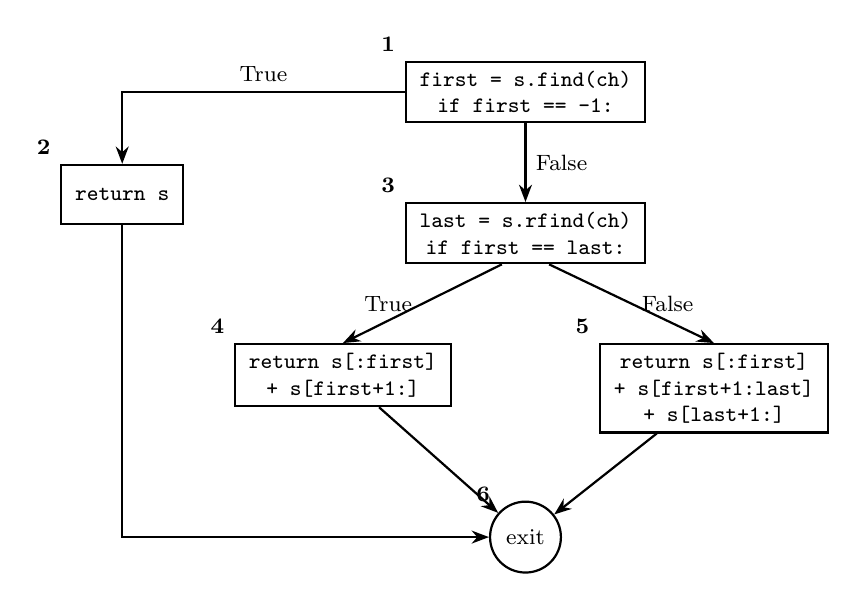
\begin{tikzpicture}[
    blk/.style={rectangle, draw=black, thick, font=\ttfamily\footnotesize, minimum height=0.75cm, inner xsep=5pt, align=center},
    ex/.style={circle, draw=black, thick, font=\footnotesize, minimum size=0.9cm},
    num/.style={font=\footnotesize\bfseries},
    e/.style={-{Stealth[length=2.2mm]}, thick},
    lab/.style={font=\footnotesize},
]
    \node[blk] (n1) {first = s.find(ch)\\if first == -1:};
    \node[blk, left=2.8cm of n1, yshift=-1.3cm] (n2) {return s};
    \node[blk, below=1.0cm of n1] (n3) {last = s.rfind(ch)\\if first == last:};
    \node[blk, below left=1.0cm and -0.6cm of n3] (n4) {return s[:first]\\+ s[first+1:]};
    \node[blk, below right=1.0cm and -0.6cm of n3] (n5) {return s[:first]\\+ s[first+1:last]\\+ s[last+1:]};
    \node[ex, below=3.0cm of n3] (n6) {exit};
    \node[num, above left=0pt of n1] {1};
    \node[num, above left=0pt of n2] {2};
    \node[num, above left=0pt of n3] {3};
    \node[num, above left=0pt of n4] {4};
    \node[num, above left=0pt of n5] {5};
    \node[num, above left=0pt of n6] {6};
    \draw[e] (n1) -| node[pos=0.25, above, lab] {True} (n2);
    \draw[e] (n1) to node[right, lab] {False} (n3);
    \draw[e] ([xshift=-3mm]n3.south) to node[left, lab] {True} (n4.north);
    \draw[e] ([xshift=3mm]n3.south) to node[right, lab] {False} (n5.north);
    \draw[e] (n2) |- (n6);
    \draw[e] (n4) to (n6);
    \draw[e] (n5) to (n6);
\end{tikzpicture}
\caption{CFG of the generated function for task 11 as constructed by the Test Executor (basic blocks 1 to 5 and the exit node 6)}
\label{fig:cfg11}
\end{figure}

\begin{table}[H]
    \centering
    \small
    \begin{tabular}{llllc}
        \toprule
        \textbf{Prime path} & \textbf{Condition} & \textbf{Test input} & \textbf{Expected output} & \textbf{Toured by} \\
        \midrule
        \texttt{[1, 2, 6]} & Character absent & \texttt{("hello", "x")} & \texttt{"hello"} & Test 1 \\
        \texttt{[1, 3, 4, 6]} & Exactly one occurrence & \texttt{("hello", "e")} & \texttt{"hllo"} & Test 2 \\
        \texttt{[1, 3, 5, 6]} & Two or more occurrences & \texttt{("hello", "l")} & \texttt{"heo"} & Test 3 \\
        \bottomrule
    \end{tabular}
    \caption{Prime paths of task 11 and the test cases that tour them, as reported by the executor}
\end{table}

The Test Case Generator produced three test cases, one per prime path, which is the minimum number required. All three predicted expected outputs were correct, and the response was accepted at the first attempt.

\subsection{Task 11: Results of the Test Executor}

\begin{table}[H]
    \centering
    \small
    \begin{tabular}{ll}
        \toprule
        \textbf{Measure} & \textbf{Value} \\
        \midrule
        Test cases generated & 3 \\
        Valid test cases & 3 \\
        \texttt{PASS} / \texttt{FAIL} / \texttt{ERROR} / \texttt{TIME LIMIT EXCEEDED} & 3 / 0 / 0 / 0 \\
        \texttt{INVALID TEST} & 0 \\
        Node coverage & 6/6 (100\%) \\
        Edge coverage & 7/7 (100\%) \\
        Edge-pair coverage & 5/5 (100\%) \\
        Prime path coverage (selected criterion) & 3/3 (100\%), criterion met \\
        Problem verdict & \texttt{PASS} \\
        \bottomrule
    \end{tabular}
    \caption{Results of the Test Executor for task 11}
\end{table}

\subsection{Task 11: Execution on a Faulty Implementation}
\label{sec:faulty}

To show that the test cases detect an incorrect implementation, the Test Executor was run on a faulty version of the generated function for task 11 (Listing~\ref{lst:faulty}). It differs from the generated function (Listing~\ref{lst:gencode}) only in line 9, where the term \texttt{+ s[last+1:]} has been removed, so that every character after the last occurrence is lost whenever the character occurs at least twice. The three test cases generated by the LLM for task 11 (Listing~\ref{lst:tests}) and the MBPP reference solution were used unchanged, and the selected criterion was prime path coverage. The executor was invoked directly, so no LLM request was issued for this run.

\begin{lstlisting}[style=python, caption={Faulty implementation of task 11 (line 9 omits \texttt{+ s[last+1:]})}, label={lst:faulty}]
def remove_Occ(s, ch):
    first = s.find(ch)
    if first == -1:
        return s
    last = s.rfind(ch)
    if first == last:
        return s[:first] + s[first+1:]
    else:
        return s[:first] + s[first+1:last]
\end{lstlisting}

The CFG of the faulty function has the same structure as that in Figure~\ref{fig:cfg11}; only the statement of node 5 differs. Table~\ref{tab:faulty} lists the outcome of each test case.

\begin{table}[H]
    \centering
    \small
    \begin{tabular}{clllllc}
        \toprule
        \textbf{Test} & \textbf{Input} & \textbf{Expected} & \textbf{Reference} & \textbf{Actual} & \textbf{Verdict} & \textbf{Test path} \\
        \midrule
        1 & \texttt{("hello", "x")} & \texttt{"hello"} & \texttt{"hello"} & \texttt{"hello"} & \texttt{PASS} & \texttt{[1, 2, 6]} \\
        2 & \texttt{("hello", "e")} & \texttt{"hllo"} & \texttt{"hllo"} & \texttt{"hllo"} & \texttt{PASS} & \texttt{[1, 3, 4, 6]} \\
        3 & \texttt{("hello", "l")} & \texttt{"heo"} & \texttt{"heo"} & \texttt{"he"} & \texttt{FAIL} & \texttt{[1, 3, 5, 6]} \\
        \bottomrule
    \end{tabular}
    \caption{Results of the Test Executor on the faulty implementation of task 11}
    \label{tab:faulty}
\end{table}

All three test cases are valid, since their expected outputs agree with the reference solution. Tests 1 and 2 follow paths that do not contain the fault and pass. Test 3 is the only test case that tours prime path \texttt{[1, 3, 5, 6]}, which executes the faulty statement in node 5; the function returns \texttt{"he"} instead of \texttt{"heo"}, and the assertion fails. Listing~\ref{lst:faultyjson} reproduces the corresponding parts of \texttt{execution\_results.json}.

\begin{lstlisting}[style=text, caption={Excerpt of the results file for the faulty implementation of task 11}, label={lst:faultyjson}]
{
  "task_id": 11,
  "function": "remove_Occ(s, ch)",
  "coverage_criterion": "Prime Path Coverage",
  "verdict": "FAIL",
  "summary": {"total": 3, "passed": 2, "failed": 1, "errors": 0, "timeouts": 0, "invalid": 0},
  "coverage": {
    "target_criterion": "Prime Path Coverage",
    "criterion_met": true,
    "node": "6/6 (100.0%)",
    "edge": "7/7 (100.0%)",
    "edge_pair": "5/5 (100.0%)",
    "prime_path": "3/3 (100.0%)",
    ...
  },
  "test_cases": [
    ...
    {
      "id": 3,
      "input": ["'hello'", "'l'"],
      "expected": "'heo'",
      "reference_output": "'heo'",
      "actual": "'he'",
      "verdict": "FAIL",
      "error": "AssertionError: expected 'heo', got 'he'",
      "path": [1, 3, 5, 6],
      "covers": [[1, 3, 5, 6]]
    }
  ]
}
\end{lstlisting}

The verdict of the problem is therefore \texttt{FAIL}, while prime path coverage is still reported as met (3/3). This illustrates that the verdict and the coverage report are independent: coverage states which paths of the code were exercised, and the verdict states whether the outputs on those paths are correct. Because the test suite tours every prime path, the fault in node 5 is necessarily executed and, in this case, revealed.

\subsection{Task 12: Results}

Task 12 requires a function that sorts a matrix in ascending order of its row sums. The generated function defines a helper function \texttt{row\_sum} inside its body and returns \texttt{sorted(M, key=row\_sum)}. Because nested helper functions are treated as single statements, the CFG consists of one basic block and the exit node, and prime path coverage reduces to the single path \texttt{[1, 2]}.

For this problem the test generation request was answered by the fallback model \breakpath{google/gemma-4-26b-a4b-it:free}. The model produced nine test cases. Eight were valid and passed; one contained the malformed argument \texttt{[[]<, []]}, which cannot be parsed, and was marked \texttt{INVALID TEST} without affecting the other test cases. All test requirements were covered, the criterion was met, and the verdict of the problem is \texttt{PASS}.

\subsection{Independent Cross-Check}

Both generated functions were compared with their reference solutions on 20,000 random inputs each, and no discrepancy was found. The two \texttt{PASS} verdicts are therefore correct.

% PLACEHOLDER: add a screenshot of the CLI output here
% \begin{figure}[H]
%     \centering
%     \includegraphics[width=0.9\textwidth]{cli_output.png}
%     \caption{Output of the command-line interface for tasks 11 and 12}
% \end{figure}

\subsection{Results for All Criteria}

Each criterion was also selected in a separate run of the pipeline. Table~\ref{tab:allcriteria} summarises the four runs; the results of each run are stored in its own output directory. The node and edge coverage runs processed task 11 only, while the edge-pair and prime path coverage runs processed tasks 11 and 12.

\begin{table}[H]
    \centering
    \small
    \begin{tabular}{lcccccc}
        \toprule
        \textbf{Criterion} & \textbf{Problems} & \textbf{PASS} & \textbf{FAIL} & \textbf{ERROR/TLE} & \textbf{Valid/total} & \textbf{Criterion met} \\
        \midrule
        Node & 1 & 1 & 0 & 0 & 13/13 & 1/1 \\
        Edge & 1 & 1 & 0 & 0 & 8/8 & 1/1 \\
        Edge-pair & 2 & 2 & 0 & 0 & 10/10 & 2/2 \\
        Prime path & 2 & 2 & 0 & 0 & 11/12 & 2/2 \\
        \bottomrule
    \end{tabular}
    \caption{Results per coverage criterion (from \texttt{summary.json} of each run)}
    \label{tab:allcriteria}
\end{table}

Table~\ref{tab:task11criteria} gives the results for task 11 in each run. Because the Code Generator is invoked anew in every run, the generated function differs between runs, and with it the CFG and the number of test requirements. In the node coverage run the generated function had only one decision (\texttt{if first == -1}) and a CFG of four nodes. In the edge-pair coverage run the first decision was the compound condition \texttt{first == -1 or last == -1}, which forms a single decision node. In every run all test cases were valid, all passed, and the selected criterion was met.

\begin{table}[H]
    \centering
    \small
    \begin{tabular}{lccccc}
        \toprule
        \textbf{Selected criterion} & \textbf{Test cases} & \textbf{Node} & \textbf{Edge} & \textbf{Edge-pair} & \textbf{Prime path} \\
        \midrule
        Node & 13 & 4/4 & 4/4 & 2/2 & 2/2 \\
        Edge & 8 & 6/6 & 7/7 & 5/5 & 3/3 \\
        Edge-pair & 4 & 6/6 & 7/7 & 5/5 & 3/3 \\
        Prime path & 3 & 6/6 & 7/7 & 5/5 & 3/3 \\
        \bottomrule
    \end{tabular}
    \caption{Task 11: number of test cases and coverage of all four criteria achieved in each run}
    \label{tab:task11criteria}
\end{table}

The number of test cases does not grow with the strength of the selected criterion: under node coverage the LLM generated 13 test cases for a CFG with four nodes, whereas under prime path coverage it generated the minimum of three. The LLM therefore does not minimise the test suite for weaker criteria, although every suite satisfied its criterion.

% ============================================================================
\section{Observations and Discussion}
\label{sec:observations}

\paragraph{Oracle problem.} The Test Case Generator predicts the expected outputs itself, so a test case is only as reliable as this prediction. Each prediction is therefore checked against the MBPP reference solution, and the generated code is executed only on confirmed test cases. The generator never sees the reference solution and is informed that the code under test may be faulty, so that it does not derive expected outputs from the code under test.

\paragraph{Necessity of automatic coverage verification.} The reasoning of the LLM about the CFG cannot be relied upon. The executor therefore constructs the CFG itself, records the test paths and checks every test requirement. Infeasible requirements cannot be recognised automatically in general and are reported as uncovered for inspection.

\paragraph{Coverage does not reveal faults of omission.} The three test cases of task 11 achieve full prime path coverage, yet a deliberately wrong implementation, \texttt{return s.replace(ch, '')}, which removes every occurrence of the character, passes all of them, because no test case contains the character three or more times. Structural coverage of the generated code exercises only the paths that exist in that code and cannot reveal behaviour that is missing from it.

\paragraph{Detection of incorrect code.} The pipeline does detect incorrect implementations. With the unchanged test cases of task 11, a faulty version that omits \texttt{+ s[last+1:]} in node 5 was reported as \texttt{FAIL} on the input \texttt{("hello", "l")} (Section~\ref{sec:faulty}), and a faulty version returning \texttt{s[:first] + s[last+1:]} was reported as \texttt{FAIL} on the input \texttt{("abcda", "a")} during verification.

\paragraph{Output formats and reasoning models.} In an earlier run, a fallback reasoning model wrote its entire reasoning (13,660 characters) into the response and was truncated before producing an answer. Responses are now accepted only if they consist exclusively of test cases, truncated responses are discarded, and malformed individual test cases, such as \texttt{[[]<, []]} in task 12, are isolated.

\paragraph{Robustness and rate limits.} Each call runs in its own process with a time limit of 10 seconds, so an infinite loop or an exception affects only one test case. The free models limit the number of requests per minute and per day; the client therefore retries once and falls back through five further models, as occurred for task 12.

% ============================================================================
\section{Conclusion}
\label{sec:conclusion}

The project implements, from first principles, a three-agent pipeline consisting of an LLM code generator, an LLM test case generator driven by a user-selected structural coverage criterion, and a deterministic test executor. The executor validates each test case against the MBPP reference solution, asserts the output of the generated function, and verifies node, edge, edge-pair and prime path coverage on the control flow graph of the generated function. The results show that coverage-driven test generation combined with independent verification yields reliable verdicts, and that structural coverage alone cannot detect missing behaviour.

% ============================================================================
\section{Member Contributions}
\label{sec:contrib}

Both members contributed equally to the design, implementation, testing and documentation of the project. Each member was responsible for one LLM agent, one part of the Test Executor, half of the supporting infrastructure and half of the report, and every module was reviewed by the member who had not written it.

\subsection*{Mayank Tanwar (IMT2023012)}
\begin{itemize}
    \item Code Generator agent (\texttt{code\_generator.py}): system and user prompts, validation of the response with \texttt{ast}, single re-prompt including the reason for the rejection.
    \item OpenRouter client and configuration (\texttt{llm\_client.py}, \texttt{config.py}): handling of rate limits and truncated responses, fallback across six free models, management of settings.
    \item Test Executor, first part (\texttt{test\_executor.py}): parser for the \texttt{<OPEN>}/\texttt{<CLOSE>} format, splitting at \texttt{\$}, evaluation of literals, validation against the reference solution.
    \item Command-line interface (\texttt{cli.py}): interactive and batch modes.
    \item Verification: runs with faulty implementations that confirmed the detection of failing and invalid test cases.
    \item Report: Sections 2 and 3 (pipeline, dataset, prompts and settings).
\end{itemize}

\subsection*{Kunal Jindal (IMT2023049)}
\begin{itemize}
    \item Test Case Generator agent (\texttt{test\_case\_generator.py}): prompts for all four coverage criteria, rule for expected outputs, strict output format and validation of the response.
    \item Coverage verification (\texttt{coverage\_probe.py}): CFG construction from the AST, recording of test paths, and verification of node, edge, edge-pair and prime path coverage.
    \item Test Executor, second part (\texttt{test\_executor.py}): worker processes per call, time limits, assertions and verdict logic.
    \item Pipeline orchestration (\texttt{pipeline.py}): loading of MBPP, sequencing of the agents, output files and \texttt{summary.json}.
    \item Verification: validation of the prime path algorithm against the textbook example and the cross-check on 20,000 random inputs against the reference solutions.
    \item Report: Sections 4 and 5 (formats, verdicts, execution results).
\end{itemize}

\end{document}
